\chapter{Security and Efficiency}
\label{Chapter4}

\begin{figure}
    \centering
    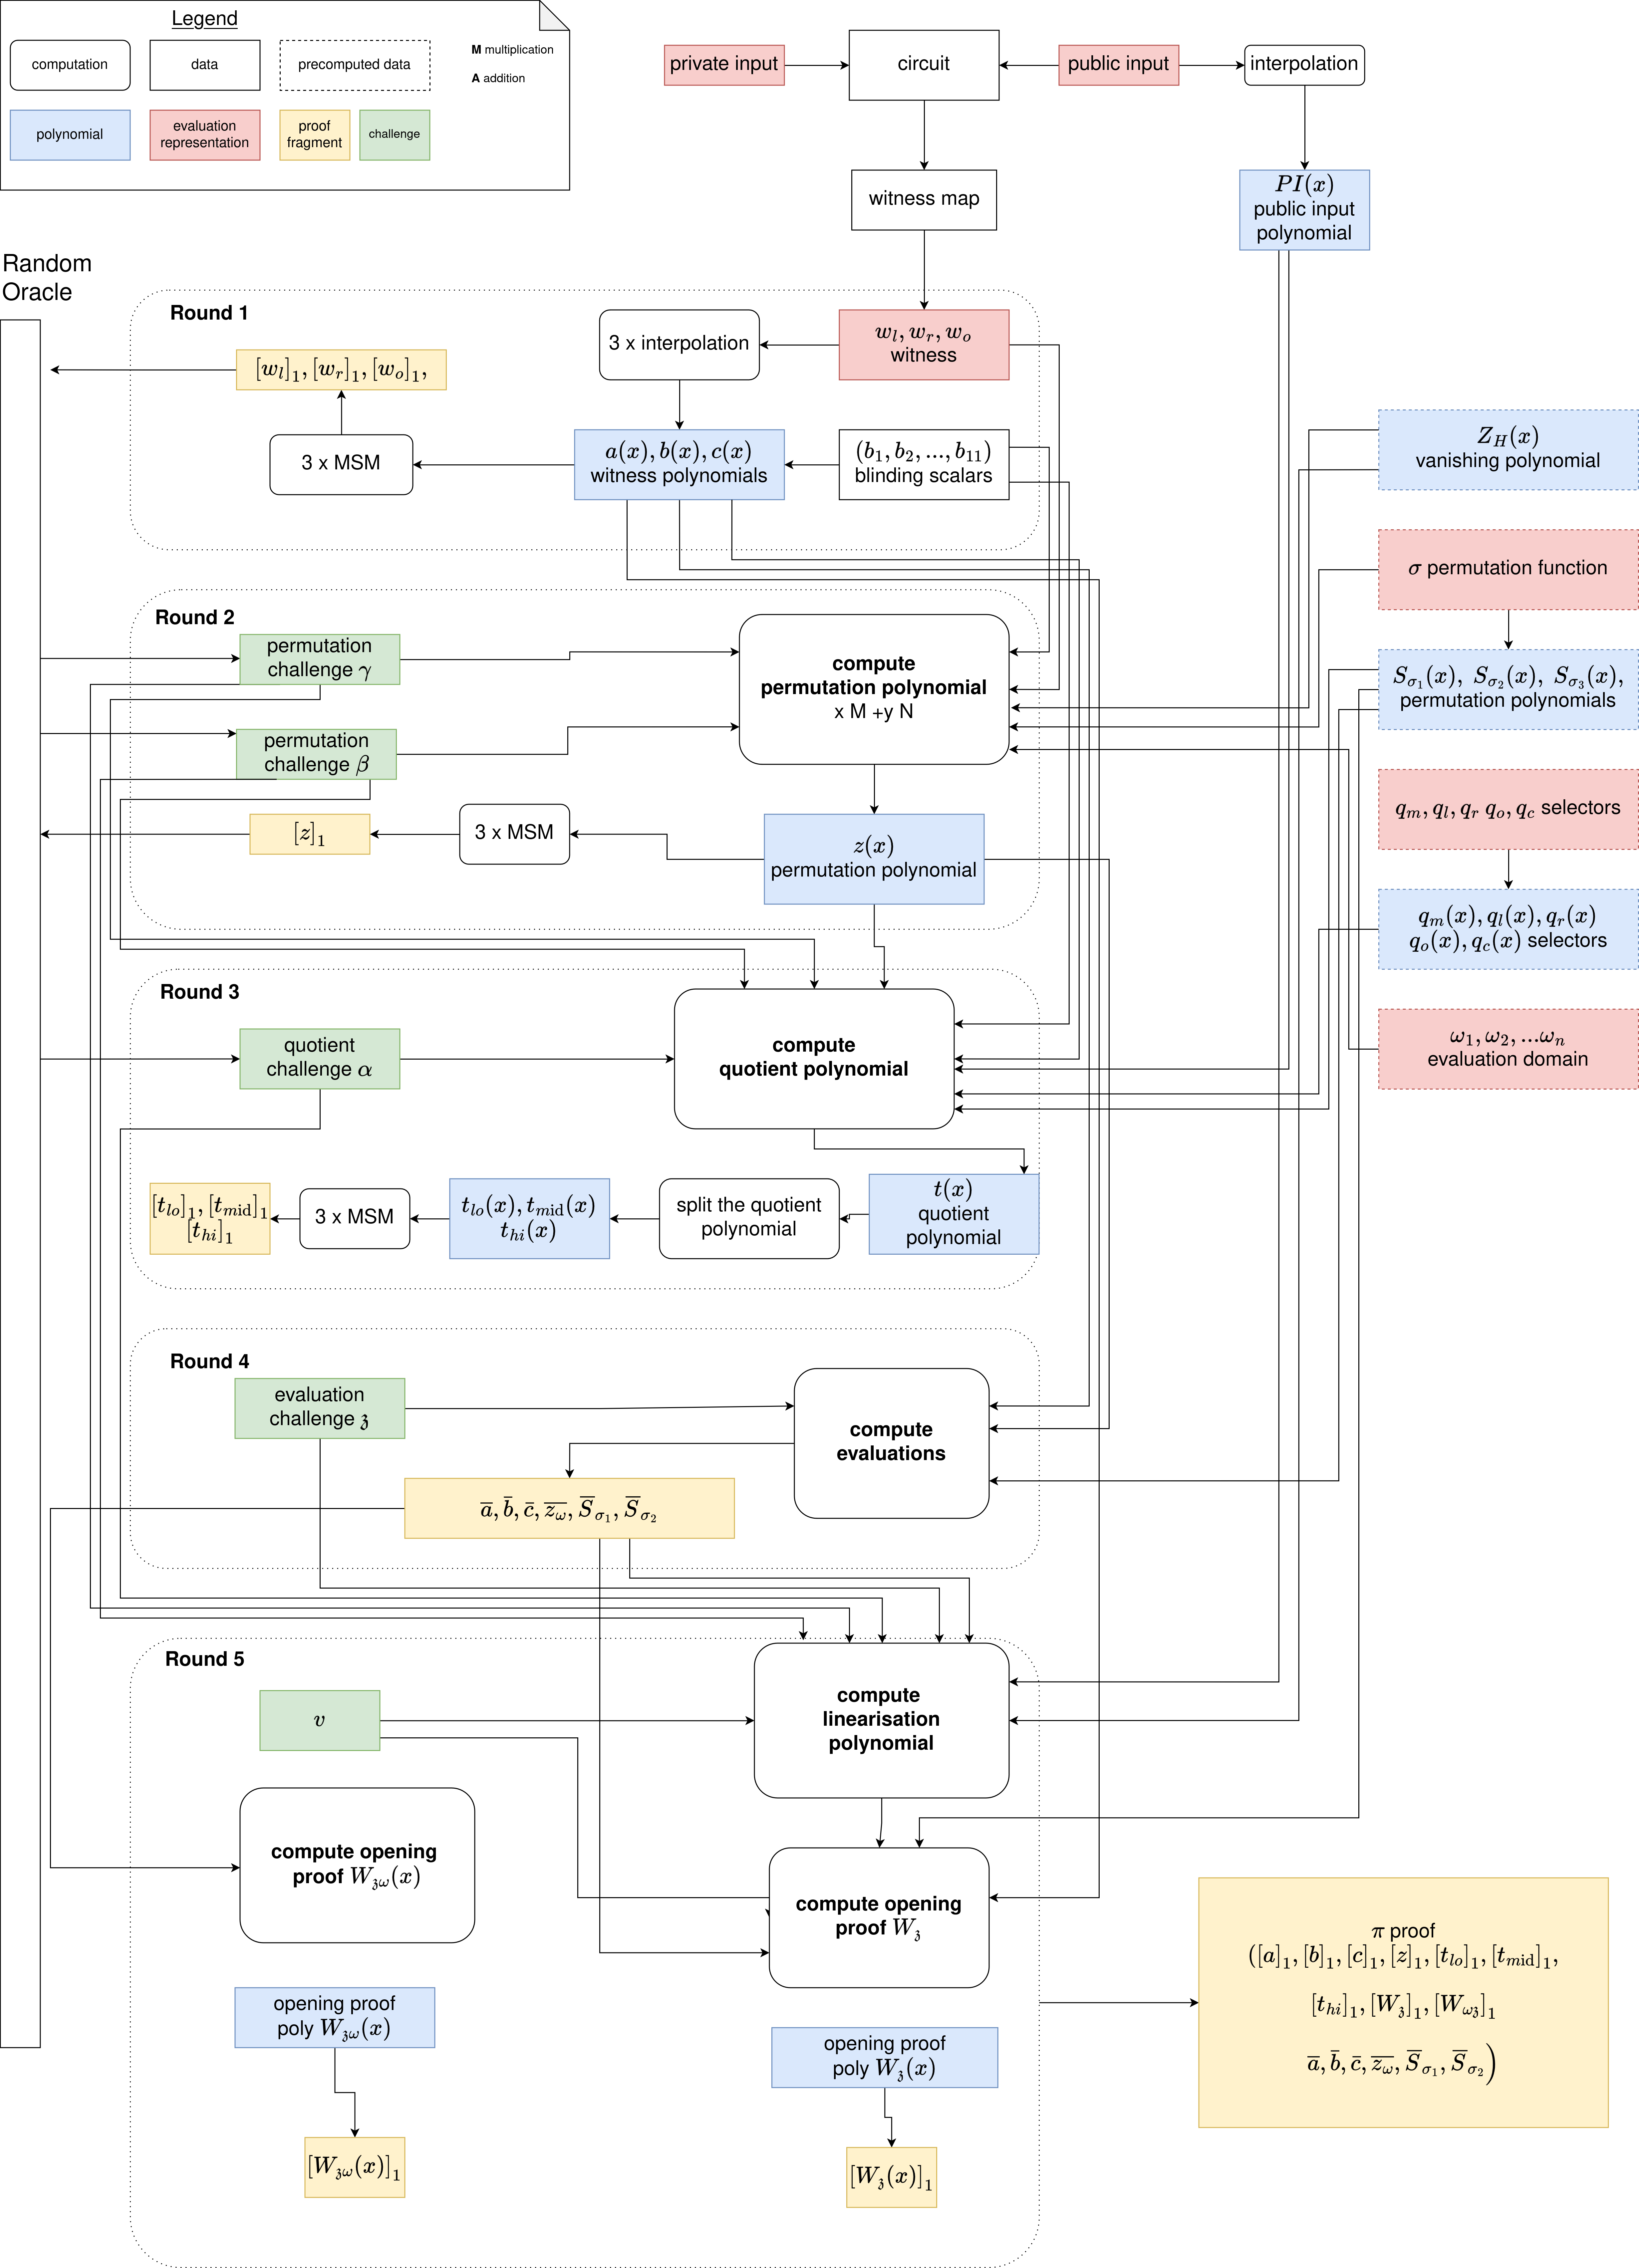
\includegraphics[width=1\linewidth]{round-figures/prover-algorithm.drawio.png}
    \caption{Enter Caption}
    \label{fig:enter-label}
\end{figure}


\section{Analysis of the protocol}

\begin{theorem}
    The PLONK Poly-IOP is a succinct non-interactive protocol that is complete, knowledge sound, and zero-knowledge.
\end{theorem}

\paragraph{Succinctness:} xxx

\paragraph{Non-Interactivity:} we have achieved by applying the \cite{fiat-shamir} Fiat-Shamir heuristic where the prover can effectively generate all of the challenges by accessing a random oracle. 

\paragraph{Completeness:} when assessing completeness we need to look at all of the properties that the proof needed to guarantee. Namely, public input check is guaranteed by xxx, circuit output check by xxx, arithmetic constraints by xxx, and wiring check by xxx.

\paragraph{Soundness:} for the soundness we again need to look at each of the constraints that need to be proven. Public input check is guaranteed by xxx, circuit output check by xxx, arithmetic constraints by xxx, and wiring check by xxx.

\paragraph{Zero-Knowledge:} In this we need to make sure that the verifier does not discover anything about the witness $w$ from the sent proof. Since the proof contains only commitments and polynomial opening it is sufficient to show that masking polynomial makes the KZG zero-knowledge which was proven by \cref{theorem:blinding}.

\section{Advantages and limitations}

The plonk protocol can run for a general circuit that has some size that is bounded by the $KZG$ setup. This setup needs to be trusted which is a downside. The computation of the protocol is still computationally expensive for the prover and the most of the time is spent with MSM and interpolation.

There is a lot of effort to make the protocol more effective most significant are the use of look-up tables in \cite{plookup} and usage of custom gates in \cite{HyperPlonk}. 



